\title{Coursework 1}
\author{Jianhong Wang\ \ \ \ CID: $01235001$}

\documentclass[12pt]{article}
\usepackage{graphicx}
\usepackage{listings}
\usepackage{amsmath}

\begin{document}
\maketitle
\textbf{Anouncement: every transition matrix and reward matrix in this answer sheet is row notation, which means row represents current state and column represents successor state.}\\
\section{Question 1}
\begin{enumerate}
\item The transition matrix for $\pi(s) = Left$ is:\\\\
\begin{tabular}{|c|c|c|c|c|c|c|c|}
\hline 
 & $s_1$ & $s_2$ & $s_3$ & $s_4$ & $s_5$ & $s_6$ & $s_7$ \\ 
\hline 
$s_1$ & 1 & 0 & 0 & 0 & 0 & 0 & 0 \\ 
\hline 
$s_2$ & 0.8 & 0.2 & 0 & 0 & 0 & 0 & 0 \\ 
\hline 
$s_3$ & 0 & 0.8 & 0.2 & 0 & 0 & 0 & 0 \\ 
\hline 
$s_4$ & 0 & 0 & 0.8 & 0.2 & 0 & 0 & 0 \\ 
\hline 
$s_5$ & 0 & 0 & 0 & 0.8 & 0.2 & 0 & 0 \\ 
\hline 
$s_6$ & 0 & 0 & 0 & 0 & 0.8 & 0.2 & 0 \\ 
\hline 
$s_7$ & 0 & 0 & 0 & 0 & 0 & 0 & 1 \\ 
\hline 
\end{tabular}\\\\\\
\newpage
The transition matrix for $\pi(s) = Right$ is:\\\\
\begin{tabular}{|c|c|c|c|c|c|c|c|}
\hline 
 & $s_1$ & $s_2$ & $s_3$ & $s_4$ & $s_5$ & $s_6$ & $s_7$ \\ 
\hline 
$s_1$ & 1 & 0 & 0 & 0 & 0 & 0 & 0 \\ 
\hline 
$s_2$ & 0 & 0.2 & 0.8 & 0 & 0 & 0 & 0 \\ 
\hline 
$s_3$ & 0 & 0 & 0.2 & 0.8 & 0 & 0 & 0 \\ 
\hline 
$s_4$ & 0 & 0 & 0 & 0.2 & 0.8 & 0 & 0 \\ 
\hline 
$s_5$ & 0 & 0 & 0 & 0 & 0.2 & 0.8 & 0 \\ 
\hline 
$s_6$ & 0 & 0 & 0 & 0 & 0 & 0.2 & 0.8 \\ 
\hline 
$s_7$ & 0 & 0 & 0 & 0 & 0 & 0 & 1 \\ 
\hline 
\end{tabular}\\\\\\
The matrix for reward function of $\pi(s) = Left$ is:\\\\
\begin{tabular}{|c|c|c|c|c|c|c|c|}
\hline 
 & $s_1$ & $s_2$ & $s_3$ & $s_4$ & $s_5$ & $s_6$ & $s_7$ \\ 
\hline 
$s_1$ & 0 & 0 & 0 & 0 & 0 & 0 & 0 \\ 
\hline 
$s_2$ & -10 & -10 & 0 & 0 & 0 & 0 & 0 \\ 
\hline 
$s_3$ & 0 & 1 & 1 & 0 & 0 & 0 & 0 \\ 
\hline 
$s_4$ & 0 & 0 & 1 & 1 & 0 & 0 & 0 \\ 
\hline 
$s_5$ & 0 & 0 & 0 & 1 & 1 & 0 & 0 \\ 
\hline 
$s_6$ & 0 & 0 & 0 & 0 & 1 & 1 & 0 \\ 
\hline 
$s_7$ & 0 & 0 & 0 & 0 & 0 & 0 & 0 \\ 
\hline 
\end{tabular}\\\\\\
The matrix for reward function of $\pi(s) = Right$ is:\\\\
\begin{tabular}{|c|c|c|c|c|c|c|c|}
\hline
 & $s_1$ & $s_2$ & $s_3$ & $s_4$ & $s_5$ & $s_6$ & $s_7$ \\ 
\hline 
$s_1$ & 0 & 0 & 0 & 0 & 0 & 0 & 0 \\ 
\hline 
$s_2$ & 0 & -1 & -1 & 0 & 0 & 0 & 0 \\ 
\hline 
$s_3$ & 0 & 0 & -1 & -1 & 0 & 0 & 0 \\ 
\hline 
$s_4$ & 0 & 0 & 0 & -1 & -1 & 0 & 0 \\ 
\hline 
$s_5$ & 0 & 0 & 0 & 0 & -1 & -1 & 0 \\ 
\hline 
$s_6$ & 0 & 0 & 0 & 0 & 0 & 10 & 10 \\ 
\hline 
$s_7$ & 0 & 0 & 0 & 0 & 0 & 0 & 0 \\ 
\hline 
\end{tabular}\\\\\\
The terminates of all of matrices above are $s_1$ and $s_7$.\\\\
\item 
\begin{align}
V(s) = \Sigma_{s^{'} \in S} P_{ss^{'}} r_{ss^{'}} + \gamma \Sigma_{s^{'} \in S} P_{ss^{'}} v(s^{'})
\end{align}
\begin{tabular}{|c|c|c|c|c|c|c|c|}
\hline 
• & $V(s_1)$ & $V(s_2)$ & $V(s_3)$ & $V(s_4)$ & $V(s_5)$ & $V(s_6)$ & $V(s_7)$ \\ 
\hline 
$initial$ & 0 & 0 & 0 & 0 & 0 & 0 & 0 \\ 
\hline 
$iteration \ 1$ & 0 & -10 & 1 & 1 & 1 & 1 & 0 \\ 
\hline 
$iteration \ 2$ & 0 & -10.5 & -0.95 & 1.25 & 1.25 & 1.25 & 0 \\ 
\hline 
$iteration \ 3$ & 0 & -10.525 & -1.1475 & 0.8725 & 1.3125 & 1.3125 & 0 \\ 
\hline
\end{tabular} 

\item The deriviation shows below:\\\\
\begin{tabular}{|c|c|c|c|c|c|c|c|}
\hline 
 & $s_1$ & $s_2$ & $s_3$ & $s_4$ & $s_5$ & $s_6$ & $s_7$ \\
\hline 
$initial$ & 0 & 0 & 0 & 0 & 0 & 0 & • \\ 
\hline 
$iteration \ 1$ & 0 & -10 & 1 & 1 & 1 & 1 & 0 \\ 
\hline 
$iteration \ 2$ & 0 & -10.5 & -0.95 & 1.25 & 1.25 & 1.25 & 0 \\ 
\hline 
$iteration \ 3$ & 0 & -10.525 & -1.1475 & 0.8725 & 1.3125 & 1.3125 & 0 \\ 
\hline 
$iteration 4$ & 0 & -10.5263 & -1.1624 & 0.8141 & 1.2401 & 1.3281 & 0 \\ 
\hline 
$iteration 5$ & 0 & -10.5263 & -1.1634 & 0.8082 & 1.2248 & 1.3144 & 0 \\ 
\hline 
$iteration 6$ & 0 & -10.5263 & -1.1634 & 0.8077 & 1.2229 & 1.3107 & 0 \\ 
\hline 
$iteration 7$ & 0 & -10.5263 & -1.1634 & 0.8077 & 1.2227 & 1.3101 & 0 \\ 
\hline
\end{tabular}\\\\
Here $\gamma$ is the same value as Question 2.\\
Meanwhile, assume that we always choose left action just as the question 1 subpart 2.
\item The full policy is:\\\\
when $p < 0.12$,\\
$\pi(Right \mid s_1) = 0$ and $\pi(Left\mid s_1) = 1$\\
$\pi(Right \mid s_2) = 1$ and $\pi(Left\mid s_2) = 0$\\
$\pi(Right \mid s_3) = 0$ and $\pi(Left\mid s_3) = 1$\\
$\pi(Right \mid s_4) = 0$ and $\pi(Left\mid s_4) = 1$\\
$\pi(Right \mid s_5) = 1$ and $\pi(Left\mid s_5) = 0$\\
$\pi(Right \mid s_6) = 1$ and $\pi(Left\mid s_6) = 0$\\
$\pi(Right \mid s_7) = 0$ and $\pi(Left\mid s_7) = 1$\\\\
when $p \geq 0.12$,\\
$\pi(Right \mid s_1) = 0$ and $\pi(Left\mid s_1) = 1$\\
$\pi(Right \mid s_2) = 1$ and $\pi(Left\mid s_2) = 0$\\
$\pi(Right \mid s_3) = 0$ and $\pi(Left\mid s_3) = 1$\\
$\pi(Right \mid s_4) = 0$ and $\pi(Left\mid s_4) = 1$\\
$\pi(Right \mid s_5) = 0$ and $\pi(Left\mid s_5) = 1$\\
$\pi(Right \mid s_6) = 1$ and $\pi(Left\mid s_6) = 0$\\
$\pi(Right \mid s_7) = 0$ and $\pi(Left\mid s_7) = 1$\\\\
$\pi(a \mid s_5)$ will change from $\pi(Right \mid s_5) = 1$ and $\pi(Left\mid s_5) = 0$ to $\pi(Right\mid s_5) = 0$ and $\pi(Left\mid s_5) = 1$ when p is greater equal than 0.12.\\
Since the state values of terminals are always zero, either action for these two states will be the optimal policy. Here we choose $\pi(Left) = 1$ to be the optimal policy for terminal states.\\
Here $\gamma$ is the same value as Question 2.\\
\end{enumerate}


\section{Question 2}
\begin{enumerate}

\item This question requests to list a return function and resolve it:\\
\begin{align}
R(T) &= r_{T+1} + \gamma r_{T+2} + ... + \gamma^{k} r_{T+k+1}\\
&= 1 + 0.8 + ... + 0.8^{k}\\
&= \frac{(1-0.8^{k+1})}{1-0.8}\\
\end{align}
Since this is an infinite sequence, so k tends to $\infty$:\\
\begin{align}
R(T) = lim_{k \rightarrow \infty} \frac{(1-0.8^{k+1})}{1-0.8} = \frac{1}{0.2} = 5
\end{align}

\item
\begin{enumerate}

\item The transition matrix should be:\\\\
\begin{tabular}{|c|c|c|c|}
\hline 
• & $Left$ & $Right$ & $Home$ \\ 
\hline 
$Left$ & $\frac{3}{7}$ & $\frac{3}{7}$ & $\frac{1}{7}$ \\ 
\hline 
$Right$ & $0$ & $\frac{1}{6}$ & $\frac{5}{6}$ \\ 
\hline 
$Home$ & 0 & 0 & $1$ \\ 
\hline 
\end{tabular}
\newpage
The reward function matrix should be:\\\\
\begin{tabular}{|c|c|c|c|}
\hline 
• & $Left$ & $Right$ & $Home$ \\ 
\hline 
$Left$ & 0 & 0 & 0 \\ 
\hline 
$Right$ & 0 & 1 & 1 \\ 
\hline 
$Home$ & 0 & 0 & 0 \\ 
\hline 
\end{tabular}\\\\\\
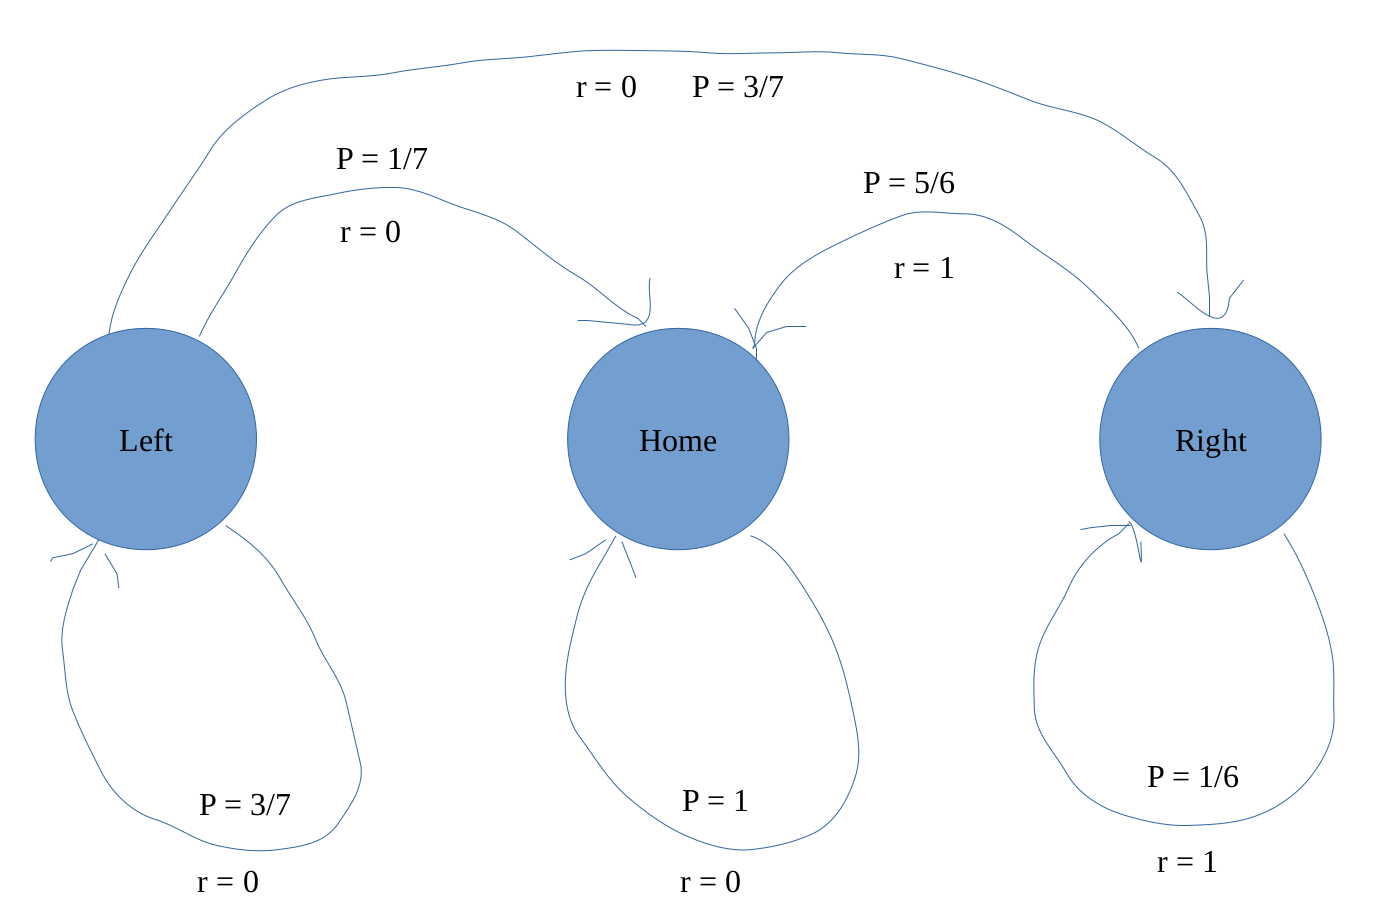
\includegraphics[scale=0.3]{q_2}\\\\\\
To infer the transition matrix, the first step is to count up the frequency from each state to another state, then computing the probability. To infer the reward function matrix, the thing is to find the immediate reward value appears in the sample for each state to another state.

\newpage
\item After observation, it can be found that:\\
\begin{align}
V(s = Right) = \frac{1}{6} \gamma V(s^{'} = Right) + 1\\
V(s = Left) = \frac{3}{7} V(s^{'} = Left) + \frac{3}{7} V(s^{'} = Right)\gamma\\
V(s = Home) = 0
\end{align}
Assume that the state value can be converged, so:\\
\begin{align}
V(s = Right) &= \frac{1}{6} \gamma V(s = Right) + 1\\
&= \frac{6}{6 - \gamma}
\end{align}
Since all of state values should converge together finally, so:\\
\begin{align}
V(s^{*} = Left) &= \frac{3}{7} V(s^{*} = Left) + \frac{3}{7} V(s^{*} = Right)\gamma\\
&= \frac{16\gamma}{7(6 - \gamma)(1 - \frac{3\gamma}{7})}
\end{align}

\end{enumerate}
\end{enumerate}

\section{Appendices}
\begin{enumerate}
\item This is the code for solving out the Question 1 subpart 3:\\
\lstinputlisting[language=Python]{q1_3.py}
\newpage
\item This is the code for solving out the Question 1 subpart 4:\\
\lstinputlisting[language=Python]{q1_4.py}
\end{enumerate}
\end{document}
